\documentclass[sigplan,10pt,anonymous,review]{acmart}\settopmatter{printfolios=true,printccs=false,printacmref=false}
%This is a template for producing LIPIcs articles. 
%See lipics-v2021-authors-guidelines.pdf for further information.
%for A4 paper format use option "a4paper", for US-letter use option "letterpaper"
%for british hyphenation rules use option "UKenglish", for american hyphenation rules use option "USenglish"
%for section-numbered lemmas etc., use "numberwithinsect"
%for enabling cleveref support, use "cleveref"
%for enabling autoref support, use "autoref"
%for anonymousing the authors (e.g. for double-blind review), add "anonymous"
%for enabling thm-restate support, use "thm-restate"
%for enabling a two-column layout for the author/affilation part (only applicable for > 6 authors), use "authorcolumns"
%for producing a PDF according the PDF/A standard, add "pdfa"

%\pdfoutput=1 %uncomment to ensure pdflatex processing (mandatatory e.g. to submit to arXiv)
%\hideLIPIcs  %uncomment to remove references to LIPIcs series (logo, DOI, ...), e.g. when preparing a pre-final version to be uploaded to arXiv or another public repository
\usepackage{stmaryrd}
\usepackage{tikz}
\usetikzlibrary{shapes,arrows}
\usetikzlibrary{intersections}
\usetikzlibrary{automata}
\usetikzlibrary{positioning}
\usepackage{booktabs}
%\graphicspath{{./graphics/}}%helpful if your graphic files are in another directory
\usepackage{listings}
\usepackage{xcolor}
\usepackage{multirow}

\lstdefinelanguage{SMTLIB}{
  morekeywords={set-logic, declare-fun, assert, check-sat, get-model},
  sensitive=true,
  morecomment=[l];,
  morestring=[b]"
}
\lstset{
  language=SMTLIB,
  basicstyle=\ttfamily\small,
  keywordstyle=\color{blue}\bfseries,
  commentstyle=\color{green!50!black},
  numbers=left,
  numberstyle=\tiny\color{gray},
  stepnumber=1,
  numbersep=5pt,
  backgroundcolor=\color{gray!10},
  frame=single,
  breaklines=true,
  captionpos=b,
  showstringspaces=false
}

\bibliographystyle{plainurl}% the mandatory bibstyle

%\titlerunning{Dummy short title} %TODO optional, please use if title is longer than one line

%%%%%%%%%%%%%%%%%%%%%%%%%%%%%%%%%%%%%%%%%%%%%%%%%%%%%%
\lstdefinelanguage{Isabelle}{
    keywords={definition,theorem,lemma,proof,qed,by,auto,simp,apply,done,
              where,fixes,assumes,shows,if,then,else,let,in,case,of,
              record,datatype,type_synonym,fun,function,primrec},
    sensitive=true,
    morecomment=[s]{(*}{*)},
    morestring=[b]",
  }

\lstset{
  language=Isabelle,
	basicstyle=\ttfamily,
	keywordstyle=\color{blue}\bfseries,
	morekeywords={definition,if,then,else,where,record,fun,lemma,type_synonym,fixes,shows,assumes,and, locale},
	escapeinside={|}{|},
  sensitive=true
}

\begin{document}

\special{papersize=8.5in,11in}
\setlength{\pdfpageheight}{\paperheight}
\setlength{\pdfpagewidth}{\paperwidth}



\title{Certified Symbolic Finite Transducers: Formalization and Applications to String Manipulation}


\begin{abstract}
    Finite Transducers (FTs) extend the capabilities of Finite Automata (FAs) by
    enabling the transformation of input strings into output strings. In many
    practical applications --- including program analysis, string constraint
    solving, and analysis of security-critical sanitizers --- Symbolic FTs 
    (SFTs) and Symbolic FAs (SFAs) are used instead of the explicitly
    represented models. To circumvent to the notorious state-space explosion 
    problem caused by the extremely large alphabet size (e.g. UTF-16), SFTs
    and SFAs allow the representation of the alphabet as an effective boolean
    algebra including finite unions of intervals, as well as 
    SMT-Algebras.
    %can be instantiated with various Boolean algebras, 
    The
    security-critical nature of many of these applications demands trustworthy
    implementations of such systems. To this end, we present the first 
    formalization of SFTs and their most important algorithms in
    Isabelle/HOL. 
    %This symbolic approach enables not only efficient FT operations—such as computing the output language of an FT given a regular language—but also supports infinite alphabets.
%
    To evaluate the effectiveness of our formalization, we apply the formalized 
    SFTs to two applications: (1) \texttt{HTMLdecode}, a sanitizer used for 
    preventing XSS attacks, and (2) string solving, which increasingly
    employs intricate string replacement operations.
    %a string solver that models replacement operations with various semantics, including left-most and replace-all matching. 
    Our experimental results demonstrate that our methods are competitive with
    the existing unverified implementations.

    %that our approach achieves computational efficiency in constraint-solving scenarios.

    %, thereby providing a more expressive framework for operations that encompass both recognition and transformation. 
%FTs have wide applications, including program analysis, string constraint 
    %solving, and security-critical sanitizer analysis. 
%However, there is currently no scalable formalization of FTs. This is primarily because transition labels in FTs are not formalized symbolically, resulting in transition explosion and significant performance bottlenecks in practical applications.

    \OMIT{
In this paper, we present a formalization of FTs in the symbolic setting using Isabelle/HOL, where transition labels can be instantiated with various Boolean algebras, such as intervals and arithmetic predicates. This symbolic approach enables not only efficient FT operations—such as computing the output language of an FT given a regular language—but also supports infinite alphabets.
%
To evaluate the effectiveness of our formalization, we apply the formalized SFTs to two applications: (1) \texttt{HTMLdecode}, a sanitizer used for preventing XSS attacks, and (2) a string solver that models replacement operations with various semantics, including left-most and replace-all matching. Experimental results demonstrate that our approach achieves computational efficiency in constraint-solving scenarios.
    }
\end{abstract}

\maketitle

\section{Introduction}
\label{sec:introduction}

Finite Automata (FA) and Finite Transducers (FT) are fundamental constructs in the theory of formal languages, with extensive applications in programming 
languages and software engineering. Despite this, many practical applications
that employ FAs and FTs --- for example, string analysis for web applications
%character sanitization in web
%applications 
(which easily prone to XSS vulnerabilities) and string constraint solving
--- require extremely large alphabets (e.g. Unicode), which are beyond the
capabilities of classical automata algorithms
\cite{DV21,cav/DAntoniV17,uss/HooimeijerLMSV11,Berkeley-JavaScript}.
More precisely, explicit automata/transducer representations would yield 
an extremely large number of transitions (potentially, one for 
each letter).
%For example, recent advancements in string solvers, as demonstrated by \cite{pacmpl/ChenFHHHKLRW22}, have illustrated the relationship between regular expressions in modern programming languages and various forms of FAs and FTs. Additionally, FAs and FTs find significant industrial applications, such as in the verification of AWS access control policies \cite{DBLP:conf/fmcad/BackesBCDGLRTV18}.



%One significant drawback from classical automata approach is that transition 
%labels are typically non-symbolic and finite. A conventional transition is represented as $q\xrightarrow{a}q'$, where $a$ is a character from a finite alphabet. This simplistic representation can lead to a phenomenon known as transition explosion. 
%For example, if the alphabet $\Sigma$ encompasses the entire Unicode range, which is common in modern programming languages, it consists of $\texttt{0x110000}$ distinct characters. Defining a transition from state $q$ to $q'$ that accepts any character in $\Sigma$ would require splitting into $\texttt{0x110000}$ individual transitions, rendering the FA and FT operations highly inefficient. Furthermore, in practical applications, it is often necessary to consider infinite alphabets, such as the set of all integers.

%Even though there are various formalizations of FAs and FTs in interactive proof assistants such as Isabelle \cite{isabelle-homepage} and Coq \cite{coq-homepage}, these are predominantly based on classical definitions. However, these traditional approaches present certain limitations when applied to practical scenarios. 



Symbolic Finite Automata (SFA) and Symbolic Finite Transducers (SFT)
\cite{cav/DAntoniV17, VeanesHLMB12Transducer,DV21} were proposed around 15 years ago
to deal with the alphabet-explosion problem that often arises in practical
applications. 
%represent advanced extensions of classic FAs and  FTs, enhancing their applicability in practical scenarios.
%
These symbolic extensions permit transition labels defined by an effective 
boolean algebra, allowing for a succinct representation of a set of transitions
that can be conveniently manipulated. 
%more expressive representations. 
For example, in the interval algebra, a transition label might be specified as 
an interval [$\texttt{a}-\texttt{z}$], encompassing all characters from
$\texttt{a}$ to $\texttt{z}$. As another example, in the SMT-Algebra
(particularly, of the theory of Linear Integer Arithmetic), %or 
one could associate an arithmetic condition ($x \mod 2 = 0$) to a transition, 
denoting all even numbers. Efficient algorithms for manipulating (e.g. computing
closures) and analyzing (e.g. checking emptiness) SFA and SFT are by now
rather mature (e.g see the CACM article \cite{DV21}).
SFA and SFT have been applied in numerous domains including analysis of web
applications against XSS vulnerabilities \cite{VeanesHLMB12Transducer,uss/HooimeijerLMSV11},
runtime behavior monitoring \cite{osdi/YaseenABCL20}, automated program
transformation \cite{pldi/HuD17}, and finally SMT solving for the unicode theory
of strings (e.g. see \cite{pacmpl/ChenFHHHKLRW22,CHL+19}).
%Furthermore, numerous studies have demonstrated the broad applicability of SFTs across diverse domains. The work of \cite{VeanesHLMB12Transducer} showcases SFTs in security-critical applications, particularly for cross-site scripting (XSS) prevention. \cite{uss/HooimeijerLMSV11} extends this security focus by applying SFTs to web application sanitizer analysis. In system verification, \cite{osdi/YaseenABCL20} employs SFTs for runtime behavior monitoring, while \cite{pldi/HuD17} demonstrates their utility in automated program transformation through systematic inversion techniques.
%This symbolic approach not only provides a more succinct representation but also supports infinite alphabets, thereby extending the expressive capabilities of FAs and FTs.

Owing to the security-critical nature of many applications of string analysis
(e.g. analysis of web applications against XSS vulnerabilities
\cite{Berkeley-JavaScript} and
at AWS for analyzing Role-Based 
Access Control (RBAC) policies \cite{neha,DBLP:conf/fmcad/BackesBCDGLRTV18}), 
there is an 
increasing need of trustworthy implementations in such application domains. 
Unfortunately, string analysis implementations are often quite buggy. For
example, even state-of-the-art SMT solvers over the theory of strings 
were found to be buggy through such techniques as fuzzing
\cite{DBLP:conf/cav/BlotskyMBZKG18,BM20,Mansur20}. 
%Recent applications of string solvers in security critical applications
%(e.g. at AWS for analyzing Role-Based 
%Access Control (RBAC) policies \cite{neha,DBLP:conf/fmcad/BackesBCDGLRTV18})
This
has motivated initial formalization efforts for the theory of strings in 
Isabelle/HOL, e.g., a verified solver \cite{cpp/KanLRS22}
for handling a small fragment of SMT-LIB 2.6 unicode theory of strings
consisting only of equality, concatenation and regular constraints, and a
formalization of the semantics of this theory \cite{verified-verifying}.

Despite these, existing verified implementations for string analysis do not
handle the following indispensable string operations for analysis of web
applications (e.g. see
\cite{DBLP:conf/popl/LinB16,Kern,Berkeley-JavaScript,systematic-transduction,uss/HooimeijerLMSV11}):
\emph{string transductions} and \emph{replaceall} operators. In particular, 
string transductions are used frequently in web applications (e.g. for
sanitization, as well as implicitly applied transductions, for instance
through \texttt{innerHTML}) and are well-known to be critical for analyzing XSS
vulnerabilities for web applications
\cite{Berkeley-JavaScript,systematic-transduction,Kern,uss/HooimeijerLMSV11,DBLP:conf/popl/LinB16}. In particular, SMT-LIB string constraints that 
arise from such applications require the \emph{replaceall} operator, which is currently not handled by any existing verified
implementation. This paper tackles the formalization of SFA/SFT and
their associated algorithms, as well as applications to analysis of sanitizers
and verified solver for string constraints. 
%\textcolor{red}{Updated up to here
%so far}

\OMIT{
SFA and SFT (e.g. 
analysis of web applications, e.g., against XSS vulnerabilities), 

However, the formalization of transition labels in SFAs and SFTs presents significant challenges within interactive proof assistants. Two fundamental considerations arise: first, the representation of transition labels must be sufficiently expressive to accommodate diverse predicate representations of boolean algebras; second, the formalization framework must be designed with extensibility in mind to facilitate the incorporation of new boolean algebras while minimizing redundant proof efforts.

}


\OMIT{
Prior work of CertiStr \cite{cpp/KanLRS22} has successfully formalized SFAs within Isabelle/HOL, demonstrating both the efficiency and effectiveness of SFAs in practice. However, the formalization of SFTs remains an open challenge, primarily due to their inherent complexity in two aspects: the formalization of transition labels and the specification of transition output functions. SFTs constitute a significantly more expressive and powerful theoretical framework compared to  SFAs, as evidenced by their capability to model complex string transformations such as replacement operations.
%
Furthermore, numerous studies have demonstrated the broad applicability of SFTs across diverse domains. The work of \cite{VeanesHLMB12Transducer} showcases SFTs in security-critical applications, particularly for cross-site scripting (XSS) prevention. \cite{uss/HooimeijerLMSV11} extends this security focus by applying SFTs to web application sanitizer analysis. In system verification, \cite{osdi/YaseenABCL20} employs SFTs for runtime behavior monitoring, while \cite{pldi/HuD17} demonstrates their utility in automated program transformation through systematic inversion techniques.
}


\paragraph{Contributions.} 
In this work, we present a comprehensive formalization of SFTs. 
%However, the formalization of transition labels in SFAs and SFTs presents significant challenges within interactive proof assistants. 
Two fundamental considerations arise in such a formalization: first, the 
representation of transition labels must be sufficiently expressive to accommodate diverse predicate representations of boolean algebras; second, the formalization framework must be designed with extensibility in mind to facilitate the incorporation of new boolean algebras while minimizing redundant proof efforts.

To address these challenges, %in supporting diverse transition label theories, 
we adopt a refinement-based approach. At the abstraction level, transition labels are formalized through the fundamental mathematical concept of \emph{sets}. This abstraction facilitates subsequent refinement to various representations of Boolean algebras, such as intervals and arithmetic predicates, while maintaining theoretical consistency.

The key operation of our formalization is the product operation between an SFT and an input regular language. Specifically, given an SFA $\mathcal{A}$ representing a regular language and an SFT $\mathcal{T}$, we define the product operation $\mathcal{T} \times\mathcal{A}$ that characterizes the output language generated by $\mathcal{T}$ when processing inputs from the language recognized by $\mathcal{A}$.


In the refinement level, we implemented transition labels using an interval-based representation to examplify the refinement process. The formalization of interval algebra provides efficient set-theoretic operations—including membership checking, intersection, and difference computations—facilitating the refinement of transition labels from abstract sets to concrete intervals. Furthermore, leveraging the data refinement framework \cite{DBLP:conf/itp/Lammich13} in Isabelle/HOL, we store states and transitions using sophisticated data structures such as hashmaps and red-black trees, ensuring efficient automata manipulation.

To evaluate the effectiveness and efficiency of our formalization, we 
provide two applications: (1) analysis of the web application sanitizers for html, css, json, and javascript
which are used for preventing XSS attacks, and (2) string solving handling equality, concatenation, regular
constraints, and more importantly the string replaceall operator, which has been
argued to be indispensable for analysis of XSS
\cite{DBLP:conf/popl/LinB16,Kern,Berkeley-JavaScript,systematic-transduction,uss/HooimeijerLMSV11}.
The experimental results demonstrate that our formalization achieves computational efficiency in constraint-solving scenarios.

\OMIT{
which increasingly
extended

the SMT-LIB \cite{smtlib} compliant certified string solver \cite{cpp/KanLRS22}
with replacement operations. We evaluated our implementation using a set of benchmarks from the SMT-LIB repository \cite{smtlib_benchmarks}.
}



In summary, our formalization makes the following contributions:
\begin{enumerate}
\item We present the first formalization of symbolic finite transducers  in Isabelle/HOL.
We prove the correctness of key operations of SFTs and symbolic SFAs, such as the product operation between SFTs and SFAs.
\item We leverage the refinement framework to develop an extensible and efficient SFT implementation capable of supporting diverse Boolean algebras, ensuring adaptability to future transition label representations. The correctness of the refined, efficient implementation is proved via structural isomorphism between refinement layers.
\item We develop a certified interval algebra with verified set-theoretic operations, enabling refinement of transition labels from abstract sets to concrete intervals.
\item We demonstrate the practical utility of our formalization by applying it to sanitizer analysis and integrating our formalized SFT into the verified forward-propagation string solver CertiStr \cite{cpp/KanLRS22}. This integration extends CertiStr from supporting only simple concatenation and regular constraints to handling more sophisticated string replacement operations.
\end{enumerate}

\paragraph{Organization.}
The remainder of this paper is organized as follows:
Section \ref{sec:motivation} provides concrete motivating examples.
Section \ref{sec:sft} introduces the definition of symbolic finite transducers and their product operations.
Section \ref{sec:formalization} presents our formalization of SFTs in Isabelle/HOL.
Section \ref{sec:application} demonstrates applications to sanitizer analysis and string constraint solving.
Section \ref{sec:related-work} discusses related work.
Section \ref{sec:conclusion} concludes and outlines future directions.


\section{Symbolic Finite Transducers}
\label{sec:sft}


We recall the definition of SFTs \cite{VeanesHLMB12Transducer}, 
abstracting from specific implementation details in Isabelle/HOL.

Let $\mathcal{U}$ be a multi-sorted carrier set or background universe, which is equipped with functions and relations over the elements. We use $\tau$ as a sort and $\mathcal{U}^\tau$ denotes the sub-universe of elements of type $\tau$.
We have a special type $\mathbb{B}$ with $\mathcal{U}^\mathbb{B} = \{ \top, \bot\}$, which corresponds to the boolean type.

A lambda term is defined as $\lambda x.~t$ of type $\tau_1 \rightarrow \tau_2$.
When $\tau_2$ is $\mathbb{B}$, this lambda term is a predicate. Let $\phi$ be a predicate. We write $a\in \llbracket\phi \rrbracket$ if $\phi~a=\top$. For non-predicate lambda terms, we view them as functions that generate output elements of type $\tau_2$ given input terms of type $\tau_1$.
With these notations and the above definitions, we can define SFTs as follows.

\begin{definition}[Symbolic Finite Transducer]
\label{def-sft}
   A Symbolic Finite Transducer over $\tau_1\rightarrow \tau_2$ is a quadruple $\mathcal{T} = (\mathcal{Q}, \Delta, \mathcal{I}, \mathcal{F})$, where 
   \begin{itemize}
   \item $\mathcal{Q}$ is a finite set of states,
   \item $\mathcal{I}\subseteq \mathcal{Q}$ is the set of initial states,
   \item $\mathcal{F} \subseteq\mathcal{Q}$ is the set of accepting states,
   \item $\Delta$ is the set of transition relations. Each element in $\Delta$ is of the form $(q, \phi, f, q')$ or written as $q\xrightarrow{\phi, f} q'$, where $q$ and $q'$ are states in $\mathcal{Q}$.
   $\phi$ is a predicate of type $\tau_1\rightarrow \mathbb{B}$.
   $f$ is a lambda term of type $\tau_1\rightarrow \tau_2$. $f$ is called an \emph{output function}.
   \end{itemize}

For each transition $q\xrightarrow{\phi, f} q'$, if there exists an element $a\in \llbracket \phi \rrbracket$, where $a$ is called an input,  then the application $(f~a)$ is the output.
   
\end{definition}

SFTs accept an input word and generate an output word. This can be defined by \emph{runs} of SFTs.
An SFT run $\sigma$ is a sequence $(q_0, \phi_0, f_0, q_1),(q_1, \phi_1, f_1, q_2),\ldots, (q_{n-1}, \phi_{n-1}, f_{n-1}, q_n)$ such that $q_0\in \mathcal{I}$ and $(q_i,
\phi_i, f_i, q_{i+1}), 0 \leq i \leq n-1$ is a transition in $\Delta$.
$\sigma$ is \emph{accepting} when $q_n \in \mathcal{F}$.

For a word $w = a_0,\ldots, a_{n-1}$, it is accepted by $\sigma$ if and only if $a_i \in \llbracket\phi_i \rrbracket$ for $0 \leq i \leq n - 1$. When $w$ is accepted, run $\sigma$ generates an output sequence $w'= f_0~a_0, \ldots, f_{n-1}~a_{n-1}$. We define:
\begin{itemize}
\item  $(a_0,(f_0~a_0)), \ldots, (a_{n-1},(f_{n-1}~a_{n-1}))$ a \emph{trace},
\item $a_0,\ldots,a_{n-1}$ the \emph{input} of the trace and $(f_0~a_0), \ldots, $ $(f_{n-1}~a_{n-1})$ the \emph{output} of the trace.
\end{itemize}

If $a_0,\ldots,a_{n-1}$ is accepted by an accepting run in $\mathcal{T}$, we say that the trace is an accepting trace of $\mathcal{T}$.
For a trace $\pi$, we denote its input as $\mathit{in}(\pi)$ and its output as $\mathit{out}(\pi)$.
%
Given an SFT $\mathcal{T}$ and a word $w$, we define the \emph{product} operation of $\mathcal{T}$ and $w$ (denoted as $\mathcal{T}\times\{w\}$) as the set of outputs generated by $\mathcal{T}$ with input $w$. More precisely,
\[
\begin{split}
\mathcal{T}\times\{w\} = \{w'\mid \exists \pi.~\pi \text{ is an accepting trace of } \mathcal{T} \land \\ \mathit{in}(\pi) = w \land \mathit{out}(\pi) = w'\}.
\end{split}
\]

To make the operation \emph{product} more general, we extend the operation to an SFT and a set of input words represented by a regular language, which can be denoted by an SFA $\mathcal{A}$. More precisely,
\[
\begin{split}
\mathcal{T}\times \mathcal{A} = \{w'\mid \exists w.~w\in \mathcal{L}(\mathcal{A})\land w' \in \mathcal{T}\times\{w\}\}, \\\text{ where }\mathcal{L}(\mathcal{A})\text{ denotes the language of }\mathcal{A}.
\end{split}
\]

\begin{figure}[hbt!]
  \centering
  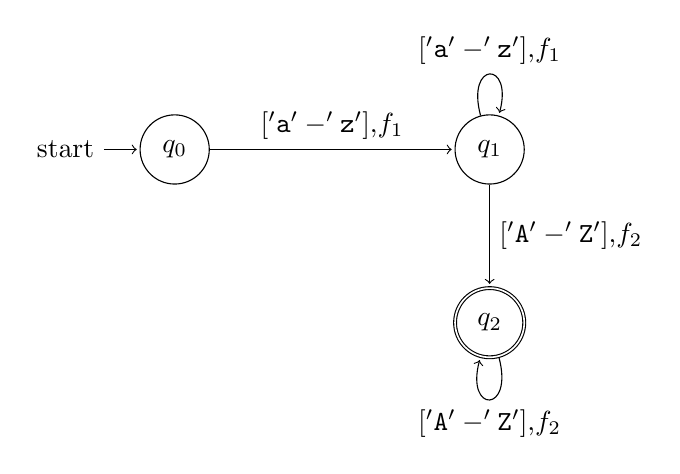
\begin{tikzpicture}[shorten >=1pt, node distance=2.5cm and 2cm, on grid, auto]
    % Make q0 and q1 horizontally wide apart
    \node[state, initial] (q_0)   {$q_0$}; 
    \node[state] (q_1) [right=4cm of q_0] {$q_1$}; 
    \node[state, accepting] (q_2) [below=2.2cm of q_1] {$q_2$}; 
 
    \path[->] 
    (q_0) edge node {[$'\texttt{a}'-'\texttt{z}'$],$f_1$} (q_1)
    (q_1) edge node[right] {[$'\texttt{A}'-'\texttt{Z}'$],$f_2$} (q_2)
    (q_1) edge[loop above] node {[$'\texttt{a}'-'\texttt{z}'$],$f_1$} (q_1)
    (q_2) edge[loop below] node {[$'\texttt{A}'-'\texttt{Z}'$],$f_2$} (q_2);
  \end{tikzpicture}
    \caption{An example of SFT}
    \label{fig-example-ft}
\end{figure}

    Figure \ref{fig-example-ft} illustrates an SFT that accepts words matching the regular expression $/['\texttt{a}'-'\texttt{z}']+['\texttt{A}'-'\texttt{Z}']+/$. The transition labels utilize intervals of the form $[i\text{-}j]$, which are interpreted as predicates $\lambda x.~i \leq x \leq j$. The output functions $f_1$ and $f_2$ perform case transformations: $f_1 = \lambda x.~\texttt{toUpper}(x)$ converts lowercase letters to uppercase, while $f_2 = \lambda x.~\texttt{toLower}(x)$ performs the inverse operation. For example, given the input string \texttt{"bigSMALL"}, this SFT produces the output \texttt{"BIGsmall"}.


%The transition labels can be more complex. For instance, it can be a predicate over integers as: $\lambda x.~ x >0 \land x \text{ mod } 2 = 0$. This symbolic label corresponds to the set of even natural numbers.


\section{The Isabelle/HOL Formalization of SFTs}
\label{sec:formalization}


In this section, we present our formalization of SFTs. We begin by outlining the basic architecture of our Isabelle/HOL formalization, which is organized into three distinct layers.

The \textbf{abstract layer} represents transition labels as \textbf{sets}, with states likewise stored in sets. This abstraction, which deliberately omits implementation details, closely aligns with the SFT definitions presented in Section~\ref{sec:sft}.

The \textbf{implementation layer} refines the abstract transition labels to a locale where a boolean algebra is defined as type variable $'\texttt{b}$ together with a collection of operations and assumptions. State sets are refined using Refine\_Monadic \cite{Refine_Monadic-AFP}, a framework in Isabelle/HOL for data refinement that automatically transforms general sets into efficient data structures such as hashmaps and red-black trees.

The \textbf{boolean algebra layer} refines the transition label locale to a concrete boolean algebra implementation. In this paper, we present an interval-based refinement.

This three-layer architecture separates the fixed components (abstract and implementation layers) of the SFT formalization from the variable components (transition labels). This separation enables us to extend the SFT formalization to accommodate new transition label theories without modifying the first two layer formalization.


\subsection{The Abstract Layer of SFTs}
\label{sec:abstract-layer}

We present the SFT formalization in abstract layer in Fig. \ref{fig-def-FT}. While the elements $\mathcal{Q}_t$, $\mathcal{I}_t$, and $\mathcal{F}_t$ directly correspond to their counterparts ($\mathcal{Q}$, $\mathcal{I}$, and $\mathcal{F}$) in Definition \ref{def-sft}, the transition relations are not exactly the same.
%
The transition relations are formalized through \texttt{LTTS} (Labeled Transducer Transition System), where each transition is represented as a triple $'q \times ('a \texttt{ set option }\times 'i) \times 'q$. This representation reflects several key design decisions aimed at enhancing the abstraction and flexibility of our SFT formalization.
\begin{figure}[hbt!]
	\begin{lstlisting}
record (|$'q,$||$~'a,$| |$'i,$| |$'b$|) |$\texttt{NFT}$| =
	|$\mathcal{Q}_t$| :: "|$'q$| set"
	|$\Delta_t$| :: "(|$'q,$||$~'a,$| |$'i$|) LTTS"
	|$\mathcal{I}_t$| :: "|$'q$| set"
	|$\mathcal{F}_t$| :: "|$'q$| set"
        |$\mathcal{M}_t$| :: "|$'i\Rightarrow ('a,~'b)$| Tlabel"
type_synonym |$('q,~'a,~'i)$| LTTS = "|$('q \times ('a \text{ set option }\times 'i) \times 'q)$| set"
type_synonym |$('a,~'b)$| Tlabel = "|$'a \text{ option}~\Rightarrow~'b$ set option"
	\end{lstlisting}
\caption{The formalization of $SFTs$ in Isabelle/HOL}
\label{fig-def-FT}
\end{figure}




Firstly, $'a \text{ set option }$ is the input type of the transition, it accepts a set of elements of type $'a$ or $\texttt{None}$ corresponding to empty string $\varepsilon$. 
Accepting a set of $'a$ elements aims to express the same but more abstract semantics of the input labels in Definition \ref{def-sft}, in which an input label is a predicate. A predicate's semantics as introduced before represents a set of elements that make the predicate true. But predicates have various different forms. For instance, the interval $[1-9]$ represents the set $\{e \mid 1 \leq e \leq 9\}$. The predicate $\lambda b.~ b[7] = 1$, where $b$ is a bit vector of length 8, denotes the set of bit vectors that have a 1 in the 7th position. All these different forms of labels are abstracted as sets in our formalization.
%
The value $\texttt{None}$ represents the empty string $\varepsilon$ in our formalization, indicating a transition that consumes no input but may still produce output elements. This design choice facilitates the modeling of real-world applications in SFTs, as we will demonstrate in our application to string solvers.

The second element of type $'i$ in LTTS serves as an index into the output function space. 
%
We use indices instead of functions themselves to enable the reuse of the same output functions for different transitions.
%
The mapping $\mathcal{M}_t$ associates each index with a specific output function. These output functions, formalized by \texttt{Tlabel}, map a single input element to a set of possible output elements rather than to a single element. This design enables non-deterministic output behavior, where the transducer may select any element from the output set randomly or according to specified criteria. Additionally, output functions can produce the empty string $\varepsilon$ by returning $\texttt{None}$, providing further flexibility in transition behavior.

%Now let us look at an example. In some modern programming languages, there are support for replacement operations : $\texttt{replace}(\texttt{str}, \texttt{pattern}, \texttt{replacement})$. This operation replaces the first occurrence of the substring  in \texttt{str} that matches \texttt{pattern} (which usually a regular expression) with the string \texttt{replacement}). 
%We can easily model this operation using our formalization of NFTs with the following steps:
%\begin{itemize}
%\item Step 1, construct a corresponding NFA from \texttt{pattern}).
%\item Step 2, convert each transition label for transducers by adding a function that maps each input character to empty, that is, generate nothing.
%\item Step 3, Add a new accepting state, and redirect existing accepting states to the new accepting state and transition label as $(\texttt{None}, \lambda x. \texttt{replacement})$.
%\item Step 4, unlabel previous accepting states as non-accepting states. 
%\end{itemize}

%We can see that the definition of transition labels in NFTs makes it is very easy to model the replacement operation.


\paragraph{The product operation formalization.} We formalize the product operation between an SFT $\mathcal{T}$ and an SFA $\mathcal{A}$, denoted as $\mathcal{T} \times \mathcal{A}$ in Section \ref{sec:sft}. The SFA is formalized as a record type \texttt{NFA in Figure \ref{fig-def-FAs}}.
An additional consideration in this operation is the presence of $\varepsilon$-transitions in our SFT formalization, which implies that the resulting automata may also contain $\varepsilon$-transitions.
%
Therefore, we need to formalize $\varepsilon$SFAs, which is shown in Fig. \ref{fig-def-FAs} as \texttt{eNFA}. The $\varepsilon$SFA formalization extends the standard SFA structure by introducing $\Delta_e'$, which captures $\varepsilon$-transitions as pairs of states, while maintaining the same labeled transition relation $\Delta$ as in standard SFAs.
In this paper, we present only the definitions of  $\varepsilon$SFAs and SFAs, while the complete formalization, including correctness proofs, is available in our Isabelle development.

\begin{figure}[hbt!]
	\begin{lstlisting}
record (|$'q,$||$~'a$|) |$\texttt{NFA}$| =
	|$\mathcal{Q}$| :: "|$'q$| set"
	|$\Delta$| :: "(|$'q,$||$~'a$|) LTS"
	|$\mathcal{I}$| :: "|$'q$| set"
	|$\mathcal{F}$| :: "|$'q$| set"

record (|$'q,$||$~'a$|) |$\texttt{eNFA}$| =
	|$\mathcal{Q}_e$| :: "|$'q$| set"
	|$\Delta_e$| :: "(|$'q,$||$~'a$|) LTS"
	|$\Delta_e'$| :: "|$('q * 'q)$| set"
	|$\mathcal{I}_e$| :: "|$'q$| set"
	|$\mathcal{F}_e$| :: "|$'q$| set"

type_synonym |$('q, 'a)$| LTS = "|$'q \times 'a \text{ set }\times 'q$|"    
	\end{lstlisting}
\caption{The formalization of $\varepsilon$SFAs and SFAs}
\label{fig-def-FAs}
\end{figure}


Having established these foundational definitions, we can now formalize the product operation. 

\begin{figure}[hbt!]
	\begin{lstlisting}
definition productT :: |$"('q,'a,'i,'b)"$| NFT |$\Rightarrow$| 
   |$('q,'a)$| NFA |$\Rightarrow$||$(('a,'b)$| Tlabel |$\Rightarrow 'a \text{ set}$| 
   |$\Rightarrow 'b\text{ set option})\Rightarrow$| |$('q\times 'q, ~'b)$| eNFA where
"productT |$\mathcal{T}$| |$\mathcal{A}$| F = |$\llparenthesis$|
  |$\mathcal{Q}e = \mathcal{Q}_t~\mathcal{T} \times \mathcal{Q} ~\mathcal{A}$|,
  |$\Delta_e = \{((p,p'),~\texttt{the }(((\mathcal{M}_t~\mathcal{T})~f)\texttt{ None}),~(q, p'))\mid $|
       |$p, p', q, f.~p'\in \mathcal{Q}~\mathcal{A}~\land$| |$(p, (\texttt{None}, f), q)\in \Delta_t~\mathcal{T}$|
        |$ \land~\exists S.~(\mathcal{M}_t~\mathcal{T})~f~\texttt{None} = \text{Some } S\} ~\cup$|
      |$\{((p,p'),~\texttt{the }(F~((\mathcal{M}_t~\mathcal{T})~f)~(\sigma_1\cap\sigma_2)),(q, q'))\mid $|
       |$p, p', q, \sigma_1, \sigma_2, q', f.~(p, (\text{Some }\sigma_1, f), q)\in \Delta_t~\mathcal{T} \land$|
       |$ (p', \sigma_2, q')\in\Delta~\mathcal{A}\land \sigma_1\cap \sigma_2 \neq \emptyset~\land$|
          |$ \exists S.~F~((\mathcal{M}_t~\mathcal{T})~f)~(\sigma_1\cap\sigma_2) = \text{Some } S\}$|,
  |$\Delta_e' = \{((p,p'),~(q, p'))\mid p, p', q, f.~p'\in \mathcal{Q}~\mathcal{A} \land$|
       |$(p, (None, f), q)\in \Delta_t~\mathcal{T}~\land $|
       |$(\mathcal{M}_t~\mathcal{T})~f~\texttt{None} = \text{None}\} ~\cup$|
      |$\{((p,p'),~(q, q'))\mid p, p', q, \sigma_1, \sigma_2, q', f.~$|
        |$ (p, (\text{Some }\sigma_1, f), q)\in \Delta_t~\mathcal{T} \land (p', \sigma_2, q')\in\Delta~\mathcal{A}$|
        |$\land~\sigma_1\cap \sigma_2 \neq \emptyset~\land\exists x\in(\sigma_1\cap\sigma_2).$|
        |$~((\mathcal{M}_t~\mathcal{T})~f)~(\text{Some } x) = \text{None} \}$|,
  |$\mathcal{I}_e = \mathcal{I}_t~\mathcal{T} \times \mathcal{I}~\mathcal{A}$|
  |$\mathcal{F}_e = \mathcal{F}_t~\mathcal{T} \times \mathcal{F}~\mathcal{A}$| |$\rrparenthesis$|"
	\end{lstlisting}
\caption{The formalization of product operation}
\label{fig-def-FTProd}
\end{figure}

Figure \ref{fig-def-FTProd} depicts the abstract level formalization for the product of an SFT and an SFA. The parameters $\mathcal{T}$ and $\mathcal{A}$ are an SFT and an SFA, respectively. The 
result of the product operation is an $\varepsilon$SFA.
But we need to explain the role of parameter $\text{\texttt{F}}$. The output function $f$ for each transition in $\Delta_t$ is of type "$'a\;\text{option} \Rightarrow 'b\;\text{set option}$", which applies to a \emph{single} element of type $'a$ or $\varepsilon$. $\text{\texttt{F}}$ extends $f$ to apply $f$ to a set of elements. More precisely, let $f$ be an output function, the semantics of $\text{\texttt{F}}$ is defined as follows:

\[\texttt{F}~f~A=\texttt{Some } (\bigcup_{a\in A} (\text{if }f~a= \text{Some }S \texttt{ then } S \texttt{ else } \emptyset))\].

The transition relations $\Delta_e$ and $\Delta_e'$ are determinted by considering two distinct cases based on the nature of transitions in the SFT: $\varepsilon$-transitions and non-$\varepsilon$-transitions. In both cases, the transition labels in the resulting $\varepsilon$SFA are derived from the composition of the SFT's output function and the SFA's input labels. Let us consider $\Delta_e$ first.

\begin{enumerate}
\item When $(p, (\text{None}, f), q)$ is a transition in $\Delta_t$, i.e. the input character is $\varepsilon$, and $f~\text{None} \neq \text{None}$. Consequently, the SFA $\mathcal{A}$ remains in its current state, and the product transition produces the output "$((\mathcal{M}_t~\mathcal{T})~f)~\text{None}$". Remember that $f$ is just an index, $(\mathcal{M}_t~\mathcal{T})~f$ is the output function.

\item When $(p, (\text{Some}~\sigma_1, f), q)$ is a transition in $\Delta_t$, synchronization is possible only with SFA transitions that share characters with $\sigma_1$, i.e., $\sigma_1\cap\sigma_2\neq \emptyset$, where $\sigma_2$ represents the input label of the corresponding SFA transition. The resulting output is $\texttt{F}~((\mathcal{M}_t~\mathcal{T})~f)~(\sigma_1\cap\sigma_2)$.
\end{enumerate}

The transitions in $\Delta_e'$ follow a similar pattern with analogous cases for $\varepsilon$ and non-$\varepsilon$ transitions.

To establish the correctness specification of the product operation, we begin by formalizing the concept of SFT \emph{traces} as introduced in Definition \ref{def-sft}. In our formalization, traces are represented by the type $('a\;\text{option} \times 'b\;\text{option})\;\texttt{list}$, as shown in Figure \ref{fig-def-output}.
%
Given a trace $\pi$, we define two key projection functions:
(1) \texttt{inputE}, which corresponds to ${in}(\pi)$ and extracts the input sequence
(2) \texttt{outputE}, which corresponds to ${out}(\pi)$ and extracts the output sequence.

The definition \texttt{outputL} generalizes \texttt{outputE} to characterize the set of all possible outputs that an SFT $\mathcal{T}$ can generate when processing inputs from the language accepted by the SFA $\mathcal{A}$. The reachability of a trace $\pi$ between states $q$ and $q'$ is checked by the predicate $\texttt{LTTS\_reachable}~\mathcal{T}~q~\pi~q'$.





\begin{figure}[hbt!]
	\begin{lstlisting}
fun inputE :: 
   "|$('a\;\text{option}\;\times\;'b\;\text{option})\;\text{list}\;\Rightarrow\;'a\;\text{list}$|"
where
  "inputE [] = []" |$\mid$|
  "inputE ((Some a, |$\_$|) |$\#$| l) = 
                      a |$\#$| (inputE l)" |$\mid$|
  "inputE ((None, |$\_$|) |$\#$| l) = (inputE l)"

fun outputE :: 
    "|$('a \text{ option} \times 'b \text{ option}) \text{ list} \Rightarrow 'b \text{ list}$|" 
where
  "outputE [] = []" |$\mid$|
  "outputE ((_,Some a) # l) = 
                    a # (outputE l)" |$\mid$|
  "outputE ((_,None) # l) = (outputE l)"

definition outputL :: 
   "|$('q, 'a, 'i, 'b)\text{  NFT} \Rightarrow 
                               ('q, 'a) \text{ NFA} \Rightarrow 'b\text{ list set}$|" where
  "outputL |$\mathcal{T}$| |$\mathcal{A}$| = {outputE |$\pi~\mid~\pi~q~q'$|. 
    |$q\in \mathcal{I}_t~\mathcal{T} \land q' \in \mathcal{F}_t~\mathcal{T}~\land$| 
    |$ \text{LTTS\_reachable }\mathcal{T}~q~\pi~q'\land$||$ \text{inputE }\pi\in \mathcal{L}~\mathcal{A}$|}"
	\end{lstlisting}
\caption{The formalization of traces in SFTs}
\label{fig-def-output}
\end{figure}


\begin{figure}[hbt!]
	\begin{lstlisting}
lemma productT_correct:
  fixes |$\mathcal{T}$| |$\mathcal{A}$| F
  assumes 
   F_ok1: "|$\forall~f~s.~(\forall e \in s.~f~(\text{Some } e) = \text{None})\longleftrightarrow$|
       |$\text{ F}~f~s = \text{None}"$|
   and F_ok2: "|$\forall~f~s.~ \texttt{F}~f~s\neq \texttt{None} \longrightarrow$| F |$f~s$| = 
        |$\text{Some }(\cup~\{\texttt{S} \mid e~\texttt{S}.~e \in s~\land~$|
        |$f~(\text{Some }e) = \text{ Some S}\})$|"
      and wfTA: "NFT_wf |$\mathcal{T}~\land \text{ NFA } \mathcal{A}$|"
  |$\textcolor{blue}{\text{shows}}$| "|$\mathcal{L}_e$| (productT |$\mathcal{T}~\mathcal{A}$| F) = outputL 
          |$\mathcal{T}~\mathcal{A}$|"

	\end{lstlisting}
\caption{The correctness lemma of the product operation}
\label{fig-def-product-correct}
\end{figure}

Figure \ref{fig-def-product-correct} presents Lemma \texttt{productT\_correct}, which establishes the correctness of the product operation. The lemma's assumptions, \texttt{F\_ok1} and \texttt{F\_ok2}, specify the essential properties of function \texttt{F}. 
The assumptions $\texttt{NFT\_wf}~\mathcal{T}$ and $\texttt{NFA}~\mathcal{A}$ ensure that the SFT $\mathcal{T}$ and the SFA $\mathcal{A}$ are well-formed.
The conclusion, marked by \textcolor{blue}{\texttt{shows}}, demonstrates that the language of the constructed $\varepsilon$SFA ($\mathcal{L}_e$ denotes the language of $\varepsilon$SFA) from $\mathcal{T} \times \mathcal{A}$ coincides with the mathematical semantics defined by \texttt{outputL}, thereby establishing semantic preservation of the product construction.

\subsection{Implementation Layer Refinement}
\label{sec_alg_refinement}
Having introduced the abstract definition of the SFT product operation in Section \ref{sec:abstract-layer}, we now turn to its algorithmic refinement. In this section, we present an efficient implementation of the product construction and refine the representation of transition labels into a Boolean algebra locale, which serves as the interface structure.


\paragraph{Boolean Algebra Locale}

Figure \ref{fig-bool-algebra-locale} presents the simplified definition of a boolean algebra locale. The type variable \texttt{'b} represents any boolean algebra, while the type variable \texttt{'a} denotes the element type of the sets that the boolean algebra represents. The locale defines a collection of operations and assumptions that characterize boolean algebra behavior, including operations for set semantics, emptiness checks, non-emptiness checks, intersection, difference, and element membership. The function "\texttt{sem}" provides the semantic interpretation of a boolean algebra as a set, with all other operations' assumptions defined in terms of this set semantics.

The locale serves as an interface to boolean algebra implementations. Any concrete boolean algebra implementation must provide a concrete instantiation of this locale, which includes defining the type variable \texttt{'b} and providing implementations for all operations along with proofs of the required assumptions.


\begin{figure}[hbt!]
\begin{lstlisting}[mathescape=true]
locale bool_algebra =
 fixes sem :: " 'b $\Rightarrow$ 'a::ord set"
 fixes empty:: "'b $\Rightarrow$ bool"
 fixes nempty:: "'b $\Rightarrow$ bool"
 fixes intersect:: "'b $\Rightarrow$ 'b $\Rightarrow$ 'b"
 fixes diff:: "'b $\Rightarrow$ 'b $\Rightarrow$ 'b"
 fixes elem:: "'a  $\Rightarrow$ 'b $\Rightarrow$ bool"
 assumes
  empty_sem: "empty s = (sem s = {})"
                                    and
  nempty_sem: "nempty s = $\neg$ (empty s)" 
                                    and
  inter_sem: "sem (intersect s1 s2) =
               (sem s1) $\cap$ (sem s2)" and
  diff_sem: "sem (diff f1 f2 s1 s2) =
               (sem s1) - (sem s2)" and
  elem_sem: "elem a s $\equiv$  (a $\in$ sem s)"
\end{lstlisting}
\caption{The boolean algebra locale}
\label{fig-bool-algebra-locale}
\end{figure}




\paragraph{Implementation layer of the product operation.} We now present the algorithmic implementation of the product operation between an SFT and an SFA\footnote{For clarity of presentation, we show a simplified version of the Isabelle/HOL implementation while preserving the essential algorithmic structure.} based on Refined\_monadic framework.

Figure \ref{fig-compute-nft-product} illustrates the core algorithm \texttt{productT\_impl}, which is implemented using the \emph{Refine\_Monadic} framework. Note that in the implementation, there are some refined operations: \texttt {nft\_tranfun}, \texttt{nfa\_states}, \texttt{nfa\_trans}, \texttt{nfa\_initial}, and \texttt{nfa\_accepting}. These are corresponding to the states, transitions, initial states, accepting states, and output function mapping of the SFT.

The operation \texttt{prods\_imp}, shown in Figure \ref{fig-def-prods_imp}, computes the Cartesian product of two state sets. This function employs the \texttt{FOREACH} construct, a higher-order iteration operator analogous to OCaml's \texttt{Set.fold}. Specifically, given a set $S$, a function $f$ of type $'a \Rightarrow 'b \Rightarrow 'b$, and an initial accumulator $I$ of type $'b$, the expression $\texttt{FOREACH}~S~f~I$ systematically applies $f$ to each element in $S$, accumulating results in a principled manner.




\begin{figure}[hbt!]
	\begin{lstlisting}
definition productT_impl where
"productT_impl |$\mathcal{T}$| |$\mathcal{A}$| F fe = do {
    Q |$\leftarrow$| prods_imp (nft_states |$\mathcal{T}$|) 
    (nfa_states |$\mathcal{A}$|);
    (D1, D2) |$\leftarrow$| trans_comp_imp 
     (nft_tranfun |$\mathcal{T}$|) F fe (nft_trans |$\mathcal{T}$|) 
      (nfa_trans |$\mathcal{A}$|) (nfa_states |$\mathcal{A}$|);
    I |$\leftarrow$| prods_imp (nft_initial |$\mathcal{T}$|)
      (nfa_initial |$\mathcal{A}$|);
    F |$\leftarrow$| prods_imp (nft_accepting |$\mathcal{T}$|) 
      (nfa_accepting |$\mathcal{A}$|);
    RETURN (Q, D1, D2, I, F)
  }"
\end{lstlisting}
\caption{The computation of SFT product}
\label{fig-compute-nft-product}
\end{figure}



\begin{figure}[hbt!]
	\begin{lstlisting}
definition prods_imp where
"prods_imp Q1 Q2 =
   FOREACH {q. q |$\in$| Q1} (|$\lambda$| q Q. do {
    S |$\leftarrow$| FOREACH {q. q |$\in$| Q2}
      (|$\lambda$| q|$'$| Q|$'$|. RETURN ({(q,q|$'$|)} |$\cup$| Q|$'$|)) |$\emptyset$|;
    RETURN (Q |$\cup$| S)
   }) |$\emptyset$|"
\end{lstlisting}
\caption{The computation of Cartesian product of two state sets}
\label{fig-def-prods_imp}
\end{figure}



\begin{figure}[hbt!]
	\begin{lstlisting}
definition trans_comp_imp where
"trans_comp_imp M F fe T1 T2 Q =
  FOREACH {t. t |$\in$| T1}
   (|$\lambda$|(q,(|$\alpha$|,f),q|$'$|) (D1,D2). 
    (if (|$\alpha$|=None) then 
     (subtrans_comp_|$\varepsilon$| M q f q|$'$| F fe 
                              T2 D1 D2)
     else
     (subtrans_comp M q (the |$\alpha$|) f 
            q|$'$| F fe T2 D1 D2))) (|$\emptyset$|, |$\emptyset$|)"
\end{lstlisting}
\caption{The computation of \texttt{trans\_comp\_imp}}
\label{fig-def-prods-imp}
\end{figure}

A central algorithmic challenge in our implementation lies in the computation of transition sets $\texttt{D1}$ (corresponding to $\Delta_e$) and $\texttt{D2}$ (corresponding to $\Delta_e'$) in Figure \ref{fig-compute-nft-product}. As shown in Figure \ref{fig-def-prods-imp}, we implement this computation through the function \texttt{trans\_comp\_imp}, which computes the synchronization of transitions between the SFT and SFA. This function decomposes the synchronization process into two distinct cases, each handled by a specialized function:

\begin{enumerate}
  \item \texttt{subtrans\_comp\_$\varepsilon$}: Processes $\varepsilon$-transitions in the SFT, where transitions consume no input but may produce output
  \item \texttt{subtrans\_comp}: Processes standard transitions in the SFT, where both input consumption and output generation may occur
\end{enumerate}




\begin{figure}[hbt!]
\begin{lstlisting}
definition subtrans_comp where
"subtrans_comp M q |$\alpha$| f q|$'$| F fe T D1 D2 =
 FOREACH {t.t|$\in$|T} (|$\lambda$| (q1,|$\alpha'$|,q1|$'$|) (D1,D2).
  (if (nempty (intersect |$\alpha$| |$\alpha'$|)) then
    do {
      D1 |$\leftarrow$| 
       (if (F (M f) (intersect |$\alpha$| |$\alpha'$|)) 
          |$\neq$| None) then
         let |$\alpha_i$| = the (F (M f) 
              (intersect |$\alpha$| |$\alpha'$|)) in
         RETURN {((q,q1), |$\alpha_i$|, (q|$'$|,q1|$'$|))} 
                |$\cup$| D1
        else RETURN D1);
      D2 |$\leftarrow$| 
       (if fe (M f) (intersect |$\alpha$| |$\alpha'$|) 
        then 
         RETURN {((q,q1), (q|$'$|,q1|$'$|))} |$\cup$| D2 
        else RETURN D2);
      RETURN (D1, D2) }
   else (RETURN (D1, D2)))) (D1, D2)"
    \end{lstlisting}
    \caption{The computation of \texttt{subtrans\_comp}}
    \label{fig-def-subtrans_comp}
    \end{figure}


    We now present the implementation of \texttt{subtrans\_comp} in detail, as shown in Figure \ref{fig-def-subtrans_comp} (the implementation of \texttt{subtrans\_comp\_$\varepsilon$} follows analogous principles). For a transtion $(q, (\text{Some}~\alpha, f), q')$ in the SFT, this function traverses all transitions in the SFA, represented by the set \texttt{T}. For each transition $(q_1, \alpha', q_1')\in \texttt{T}$, the function performs two key operations when the intersection of input labels is non-empty ($\alpha \cap \alpha' \neq \emptyset$, verified using \texttt{nemptyIs}):

    \begin{enumerate}
      \item Computes non-$\varepsilon$-transitions ($\texttt{D1}$): When the output function applied to the intersection $\alpha \cap \alpha'$ yields a non-empty set, a new transition is added to $\texttt{D1}$ with the computed output label.
      \item Generates $\varepsilon$-transitions ($\texttt{D2}$): When there exists at least one input in the intersection $\alpha \cap \alpha'$ that produces an empty string (verified by checking if $\texttt{M}~f$ maps any element to \texttt{None}. The checking is implemented by \texttt{fe}), a corresponding $\varepsilon$-transition is added to $\texttt{D2}$.
    \end{enumerate}
    

  \begin{figure}[hbt!]
    \begin{lstlisting}
  lemma productT_imp_correct:
  assumes finite_TT: "|$\text{finite } (\Delta_t~\mathcal{T})$|"
      and finite_TA: "|$\text{finite } (\Delta~\mathcal{A})$|"
      and finite_Q: "|$\text{finite } (\mathcal{Q}~\mathcal{A})$|"
      and finite_TQ: "|$\text{finite } (\mathcal{Q}_t~\mathcal{T})$|"
      and finite_I: "|$\text{finite } (\mathcal{I}~\mathcal{A})$|"
      and finite_TI: "|$\text{finite } (\mathcal{I}_t~\mathcal{T})$|"
      and finite_F: "|$\text{finite } (\mathcal{F}~\mathcal{A})$|"
      and finite_TF: "|$\text{finite } (\mathcal{F}_t~\mathcal{T})$|"
  shows "|$\text{productT\_imp } \mathcal{T}~\mathcal{A}~F~\text{fe}\leq$|
            |$\text{SPEC } (\lambda A.~A = \text{productT } \mathcal{T}~\mathcal{A}~F)$|"
  \end{lstlisting}
  \caption{The refinement relation between \texttt{productT\_imp} and \texttt{productT}}
  \label{fig-def-productT_imp_correct}
  \end{figure}

  The correctness of the product computation is established through a refinement proof, demonstrating that \texttt{productT\_imp} (Figure \ref{fig-compute-nft-product}) correctly implements the abstract specification \texttt{productT} (Figure \ref{fig-def-FTProd}). This refinement relationship is formally specified in Figure \ref{fig-def-productT_imp_correct}, where we leverage the \emph{Refine\_Monadic} framework's data refinement.

  The refinement is expressed through the relation $\mathbf{C} \leq \texttt{SPEC}~\mathbf{A}$, which asserts that the concrete implementation $\mathbf{C}$ is an element of the abstract specification $\mathbf{A}$. More precisely,  the concrete implementation must produce an $\varepsilon$SFA that is structurally equivalent or isomorphic to the one produced by the abstract algorithm \texttt{productT}.

  To establish this equivalence, we must prove that the $\varepsilon$SFAs produced by \texttt{productT\_imp} and \texttt{productT} are isomorphic in all essential components: the set of states, transition relations, $\varepsilon$-transition relations, initial and accepting state sets.



The implementation of \texttt{productT\_imp} takes advantages of \emph{Refine\_Monadic} framework's interfaces for sets to store states and transition relations. 
The \emph{Refine\_Monadic} framework provides a way to automatically refine these interfaces to more efficient data structure, such as red-black trees or hashmaps. 
In our formalization, we refine the sets of storing states and transitions to red-black trees.

\subsection{Interval Implementation}

Finally, we present the implementation of the interval algebra which implements all operations defined in boolean algebra locale.
An interval is defined as a pair $(i, j)$ (represented as $[i-j]$ as well in the paper) representing the set $\{e \mid i \leq e \leq j\}$. To achieve greater expressiveness, our formalization extends this notion to interval lists of the form $[(i_1, j_1), \ldots, (i_n, j_n)]$, which denote the set $\bigcup_{1\leq k\leq n}\{e \mid i_k \leq e \leq j_k\}$. This generalization offers two key advantages: it enables more compact representation of transitions in SFAs and SFTs through merging, and it allows for efficient handling of interval operations without unnecessary splitting. For example, the set difference between intervals $(1, 5)$ and $(3, 4)$ can be directly represented as the interval list $[(1, 2), (5, 5)]$, which is also an interval.


Throughout the following discussion, we use the term "interval" to refer to interval lists. Our formalization provides all operations in the boolean algebra locale. For instance, we implement \texttt{intersect} for intervals, which computes the intersection of two intervals $i_1$ and $i_2$, yielding an interval $i$ such that $\texttt{sem}~i = \texttt{sem}~i_1 \cap \texttt{sem}~i_2$

To facilitate formal reasoning and optimize performance, in addition to the above locale operations, we introduce a canonical form for interval. An interval $[(i_1, j_1), $ $\ldots, (i_n, j_n)]$ is in canonical form if it satisfies two key properties:
\begin{enumerate}
  \item Each $(i_k, j_k)$ is well-formed: $i_k \leq j_k$ for all $k \in \{1,\ldots,n\}$
  \item Intervals are ordered and non-overlapping: $j_k < i_{k+1}$ for all $k \in \{1,\ldots,n-1\}$
\end{enumerate}

We prove that all interval operations preserve canonical form when applied to canonically-formed inputs. This invariant serves two purposes: it simplifies formal proofs by eliminating the need to reason about malformed or overlapping intervals, and it enables more efficient implementations of interval operations by reducing the number of cases to consider.


\section{Applications and Evaluation}

We evaluate our formalization and implementation of the SFT product operation in two key application domains: string sanitization and string replacement operations in string solving. These applications demonstrate the practical utility of our certified SFT product operation in real-world scenarios.
\subsection{Sanitizer}

An important application of our formalization lies in string sanitization for web applications. Sanitizers are crucial for preventing security vulnerabilities such as cross-site scripting (XSS) attacks by ensuring that user inputs are properly encoded before rendering in web browsers. Listing \ref{lst-html-encode} presents a C\# code snippet implementing an HTML encoding function—a fundamental sanitization operation. This function iterates through each character in the input string and encodes characters that are unsafe for HTML rendering.



\begin{lstlisting}[language={[Sharp]C}, caption={C\# Code for AntiXSS.EncodeHtml version 2.0.}, label={lst-html-encode}, float=htbp]
static string EncodeHtml(string t)
{
  if (t == null) { return null; }
  if (t.Length == 0) {
    return string.Empty;
  }
  StringBuilder builder = new
    StringBuilder("", t.Length * 2);
  foreach (char c in t) {
    if ((((c > ''') && (c < '{')) |$\mid\mid$|
         ((c > '@') && (c < '['))) |$\mid\mid$|
         (((c == ' ') || ((c > '/') && (c < ':'))) |$\mid\mid$|
         (((c == '.') || (c == ',')) |$\mid\mid$|
         ((c == '-') || (c == '_'))))) {
          builder.Append(c);
      }
      else {
          builder.Append("&#" +
          ((int) c).ToString() + ";");
      }
  }
  return builder.ToString();
}
\end{lstlisting}

Figure \ref{fig:html-sanitizer-sft} illustrates the SFT representation of the HTML encoding sanitizer function. The transducer accepts any input string and produces an output where safe characters are preserved using the identity function $\texttt{id}$, while unsafe characters are encoded as HTML entities. The set of safe characters is defined as $\texttt{safe\_chars} = [\texttt{' '}, \texttt{','}, \texttt{'.'}, \texttt{'-'}, \texttt{'\_'}] \cup [\texttt{'0'}-\texttt{'9'}] \cup [\texttt{'A'}-\texttt{'Z'}] \cup [\texttt{'a'}-\texttt{'z'}]$, which can be efficiently represented using the interval algebra we formalized. Unsafe characters are transformed using the encoding function $\texttt{encode}(c) = \texttt{``\&\#''} + \texttt{toString}(\texttt{ord}(c)) + \texttt{``\;''}$. When the alphabet is set to Unicode $[\mathtt{0x0000}, \mathtt{0x10FFFF}]$, the complement $\neg\texttt{safe\_chars}$ represents all Unicode characters outside the safe set, which can also be efficiently represented using our formalized interval operations.
\begin{figure}[htbp]
\centering
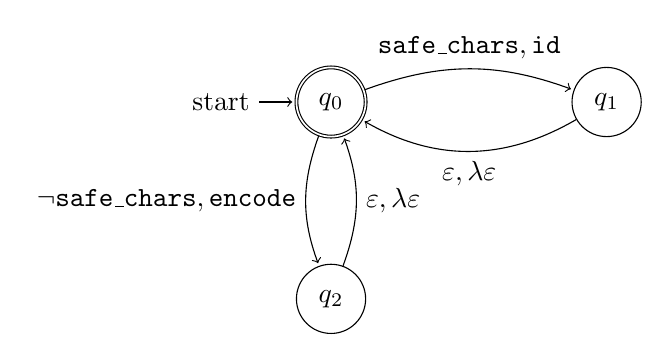
\begin{tikzpicture}[shorten >=1pt, node distance=2.5cm, on grid, auto]
  % States
  \node[state, initial, accepting] (q0) {$q_0$};
  \node[state] (q1) [right=3.5cm of q0] {$q_1$};
  \node[state] (q2) [below=of q0] {$q_2$};
  
  \path[->] 
    % Transition for safe characters
    (q0) edge[bend left=20] node[above,midway=1] {$\texttt{safe\_chars}, \texttt{id}$} (q1)
    % Transition for unsafe characters  
    (q0) edge[bend right=20] node[left,midway] {$\neg\texttt{safe\_chars}, \texttt{encode}$} (q2)
    % Epsilon transitions back to q0
    (q1) edge[bend left=30] node[below,midway] {$\varepsilon, \lambda\varepsilon$} (q0)
    (q2) edge[bend right=20] node[right,midway] {$\varepsilon, \lambda\varepsilon$} (q0);
\end{tikzpicture}
\caption{SFT representation of the HTML encoding sanitizer function.}
\label{fig:html-sanitizer-sft}
\end{figure}

We evaluate the performance of our SFT product operation by computing the product of the HTML encoding sanitizer SFT with SFAs constructed from randomly generated Unicode user inputs. This experimental setup reflects realistic usage scenarios where diverse character sets and input patterns are encountered. The experimental evaluation was conducted on a laptop with an Apple M4 processor and 24 GB of memory, with a one-minute time limit per test.

Figure \ref{fig:benchmark-results} demonstrates the scalability characteristics of our SFT product implementation. The computation requires approximately 1 second for 100,000-character inputs and 10 seconds for 1,000,000-character inputs. These performance metrics confirm that our certified implementation maintains computational efficiency suitable for practical string processing applications at scale.

\begin{figure}
\centering
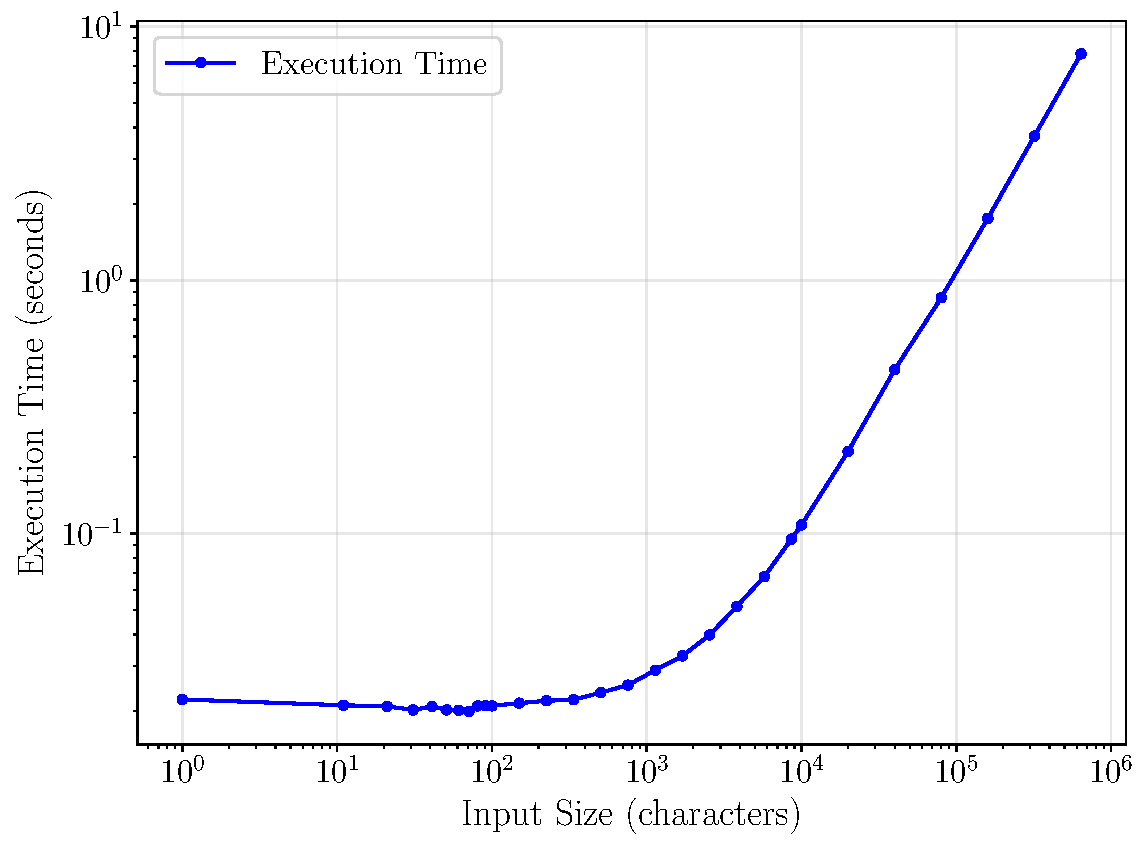
\includegraphics[scale=0.45]{benchmark_loglog.pdf}
\caption{Experimental results for the sanitizer product}
\label{fig:benchmark-results}
\end{figure}

Beyond performance evaluation, our SFT formalization enables formal verification of string sanitizer correctness. A santizer is used to transform user inputs into safe outputs, ensuring that the output does not contain any unsafe characters. However, santizers just like programs, which are eror-prone. Manual reviews of sanitizers are often insufficient to guarantee correctness.

Based on our formalization, we can verify sanitizers by modeling the sanitizer as an SFT and the user input as an SFA. We can also model potential attacks as SFAs that accept unsafe strings. Formally speaking, Let $\mathcal{T}$ be an SFT, $\mathcal{I}$ is the possible user inputs modeled by an SFA, and $\mathcal{A}$ is the attack SFA that accepts unsafe strings. The santizer correctness checking against the attack is to check whether the intersection of the product $\mathcal{T} \times \mathcal{I}$ and the attack SFA $\mathcal{A}$ is empty, i.e., $\mathcal{T} \times \mathcal{I} \cap \mathcal{A} = \emptyset$.

Moreover, santizers are usually used in combination with other sanitizers to ensure comprehensive safety. For example, the HTML encoding sanitizer can be combined with a string trimming operation to remove leading and trailing whitespace characters. For this kind of sanitizer composition, it can be modeled by our SFT product as well. Let $\mathcal{T}_1$ and $\mathcal{T}_2$ correspond to two sanitizers, and $\mathcal{T}_1$ is applied before $\mathcal{T}_2$. What we need to check is $\mathcal{T}_2 \times (\mathcal{T}_1 \times \mathcal{I}) \cap \mathcal{A} = \emptyset$.




\begin{table}[h]
  \centering
  \small
  \setlength{\tabcolsep}{4pt} % Reduced column gap
  \begin{tabular}{p{2.2cm}ll} % Increased width for automatic line break
    \toprule
    \textbf{Attack Model} & \textbf{Verfication Result} & \textbf{Size} \\
    \midrule
    attack\_html           & GA HtmlEscape: \textbf{Unsafe} & 1/6\\
                           & Trim + GA HtmlEscape: \textbf{Safe} & 4/12 \\
                           & escapeString: \textbf{Unsafe} & 1/11 \\
                           & Trim + escapeString: \textbf{Safe} & 4/17 \\
                           & Trim + OWASP HTMLEncode: \textbf{Safe} & 4/18 \\
    \midrule
    attack\_javascript     & GA Htmlescape + GA PreEscape + & 3/20 \\
                           &  gaSnippetesc: \textbf{safe} & \\
    \midrule
    attack\_json           & Trim + GA JSONESc : \textbf{Safe} & 4/16\\
    \midrule
    attack\_xml            & Trim + GA XMLEsc: \textbf{safe} & 4/16\\
    \midrule
    attack\_ccs            & Trim + GA CleanseCSS : \textbf{Safe} & 25/46\\
    \bottomrule
  \end{tabular}
  \caption{Sanitizer verfication result}
  \label{tab:sanitizer_attack}
\end{table}

Table \ref{tab:sanitizer_attack} summarizes the verification results for various sanitizers against different attack models. The first column lists the attack models, the second column indicates whether the sanitizer is classified as safe or unsafe with respect to the attack, and the third column reports the size of the transducers used in the verification, given as [number of states/number of transitions]. For composed SFTs, the size reflects the total number of states and transitions across all components.

We evaluate a range of attack models for HTML, JavaScript, JSON, XML, and CSS. Listing \ref{lst-css-attack} shows the CSS attack model, which is used to verify the corresponding sanitizer. The attack model includes comments, declaration breakers, and known dangerous tokens such as \textbf{expression(}, \textbf{@import}, \textbf{behavior:}, \textbf{-moz-binding}, and \textbf{url(} (unless the URL is separately validated). Sanitizers include GA HtmlEscape, GA JSONEscape, GA XMLEscape, escapeString, and GA CleanseCSS, where "GA" means from Google. Sanitizers are often composed with preprocessing steps such as Trim, which removes leading and trailing whitespace characters. As shown in the table, GAHtmlEscape and escapeString are unsafe with respect to the HTML attack model without preprocessing, but become safe when combined with Trim. The \textbf{Size} column demonstrates the expressive power and succinctness of SFTs in modeling real-world transducers. We did not list the execution time of verification because all of them are quite efficent with less than 0.02 second to finish the verificaiton.




\begin{lstlisting}[language={}, caption={CSS attack model for sanitizer verification.}, label={lst-css-attack}, float=htbp]
|$\Sigma$|* ( / \* [\s\S]*? \*/
  |$\mid$| ; |$\mid$| \{ |$\mid$| \}
  |$\mid$| [eE][xX][pP][rR][eE][sS][sS][iI]
    [oO][nN]\s*\(
  |$\mid$| @\s*[iI][mM][pP][oO][rR][tT]
  |$\mid$| [bB][eE][hH][aA][vV][iI][oO][rR]\s*:
  |$\mid$| -\s*[mM][oO][zZ]-\s*[bB][iI][nN]
    [dD][iI][nN][gG]
  |$\mid$| (?!allowUrl) [uU][rR][lL]\s*\(
 ) |$\Sigma$|*
\end{lstlisting}

\subsection{Modeling the Replacement Operation}

The string replacement operation, denoted as
$\texttt{replace}(\texttt{str}, \newline\texttt{pattern}, \texttt{replacement})$, is a fundamental string transformation that takes three parameters:
\begin{itemize}
  \item $\texttt{str}$: The input string to be transformed.
  \item $\texttt{pattern}$: A regular expression defining the matching criteria.
  \item $\texttt{replacement}$: The string to be substituted for the matched substring.
\end{itemize}

The semantics of the replacement operation can be formally characterized by two distinct cases:
\begin{enumerate}
  \item When there exists at least one substring $s'$ in \texttt{str} such that $s'$ matches $\texttt{pattern}$, then $s'$ is replaced with \texttt{replacement}.
  \item When no substring of \texttt{str} matches $\texttt{pattern}$, the operation returns \texttt{str} unchanged.
\end{enumerate}

The first case can be modeled by SFTs. We illustrate this case by an example. Given a replacement operation $\texttt{replace}\newline(s, \texttt{/[0-9]+/}, "\texttt{NUM}")$, which means replacing a occurrence of the substring that matches the regular expression $\texttt{/[0-9]+/}$ with the string "\texttt{NUM}".
We model this replacement operation by an SFT with the following 3 steps:

\begin{enumerate}
  \item First, construct an SFA that recognizes the regular expression pattern $\texttt{/[0-9]+/}$. Transform this SFA into an SFT by augmenting each transition with an output function $f = \lambda x.~\texttt{None}$ that produces the empty string. 
  \item Second, construct an SFA that accepts the replacement string "\texttt{NUM}". Since a constant string can be viewed as a specialized regular expression, we can construct its SFA representation. Convert this SFA into an SFT by adding $\varepsilon$-transitions  and appropriate output functions that emit the characters of "\texttt{NUM}" in sequence.
  \item Finally, compose the two SFTs through concatenation and augment the resulting transducer with self-loop transitions at the initial and final states. These additional transitions, labeled with $\Sigma$ (the set of all characters in the alphabet) and the identity function $\texttt{id}=\lambda x.~x$, enable the SFT to process arbitrary prefixes and suffixes of the input string while preserving the replacement behavior on matched substrings.
\end{enumerate}


\noindent\emph{Step 1.}
Figure \ref{fig-snfa-pattern} illustrates the construction of the pattern-matching component. The left side shows the SFA that recognizes the regular expression $\texttt{/[0-9]+/}$, while the right side presents its transformation into an SFT. This transformation is achieved by augmenting each transition with the output function $\texttt{f} = \lambda x.~\texttt{None}$, which consistently produces the empty string, effectively "consuming" the matched digits without generating output.





\begin{figure}[h] \centering
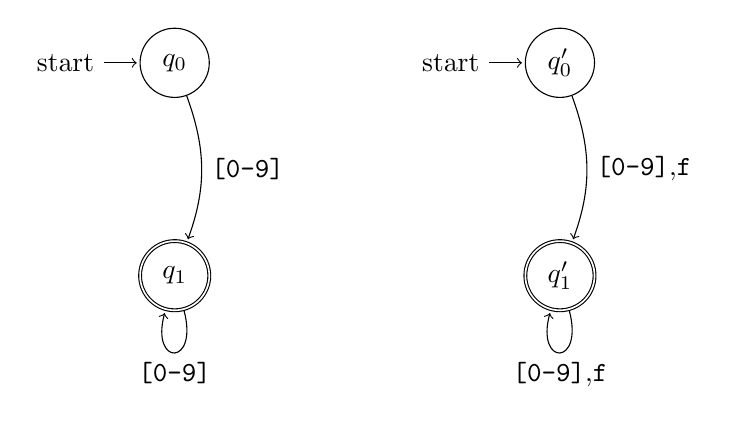
\begin{tikzpicture}[shorten >=1pt, node distance=1.8cm, auto]
  % Left: SFA for [0-9]+ (vertical)
  \node[state, initial] (q0)   {$q_0$}; 
  \node[state, accepting, below=of q0] (q1) {$q_1$}; 

   \path[->] 
   (q0) edge [bend left=20] node[right] {\texttt{[0-9]}} (q1)
   (q1) edge [loop below] node {\texttt{[0-9]}} (q1);

  % Right: SFT for [0-9]+ (vertical)
  \node[state, initial, right=4cm of q0] (q0') {$q_0'$}; 
  \node[state, accepting, below=of q0'] (q1') {$q_1'$}; 

   \path[->] 
   (q0') edge [bend left=20] node[right] {\texttt{[0-9]},$\texttt{f}$} (q1')
   (q1') edge [loop below] node {\texttt{[0-9]},$\texttt{f}$} (q1');
\end{tikzpicture}
\caption{Corresponding SFA and SFT for \texttt{/[0-9]+/}}
\label{fig-snfa-pattern}
\end{figure}

\noindent\emph{Step 2.}
Figure \ref{fig-snfa-replacement} depicts the automata for the replacement string "\texttt{NUM}". The left side shows the SFA that accepts this constant string, while the right side presents its SFT transformation. The transformation employs an indexed output function \texttt{g} that emits characters of the replacement string sequentially:
\[
\texttt{g} = \lambda~i~x.~\texttt{match}~i~\texttt{with}~
\begin{cases}
1 \mapsto [(78, 78)] & \text{(ASCII for 'N')} \\
2 \mapsto [(85, 85)] & \text{(ASCII for 'U')} \\
3 \mapsto [(77, 77)] & \text{(ASCII for 'M')} \\
\_ \mapsto \texttt{None}
\end{cases}
\]
This function maps transition indices to their corresponding character outputs, using ASCII codes to represent the string "\texttt{NUM}" character by character.


\begin{figure}[h] \centering
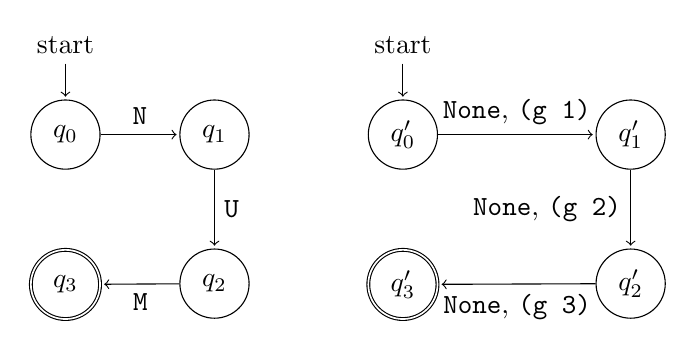
\begin{tikzpicture}[shorten >=1pt, node distance=2cm, auto]
  % SFA for "NUM" (top)
  \node[state, initial above] (q0)   {$q_0$}; 
  \node[state] (q1) [right=1cm of q0] {$q_1$}; 
  \node[state] (q2) [below=1cm of q1] {$q_2$}; 
  \node[state, accepting] (q3) [below=1cm of q0] {$q_3$}; 

  \path[->] 
  (q0) edge node {\texttt{N}} (q1)
  (q1) edge node {\texttt{U}} (q2)
  (q2) edge node {\texttt{M}} (q3);

  % SFT for "NUM" (right)
  \node[state, initial above] (q0') [right=1.5cm of q1] {$q_0'$}; 
  \node[state] (q1') [right=of q0'] {$q_1'$}; 
  \node[state] (q2') [below=1cm of q1'] {$q_2'$}; 
  \node[state, accepting] (q3') [below=1cm of q0'] {$q_3'$}; 

  \path[->] 
  (q0') edge node {\texttt{None}, \texttt{(g 1)}} (q1')
  (q1') edge node[left] {\texttt{None}, \texttt{(g 2)}} (q2')
  (q2') edge node[below] {\texttt{None}, \texttt{(g 3)}} (q3');
\end{tikzpicture}
\caption{Corresponding SFA and SFT for "\texttt{NUM}"}
\label{fig-snfa-replacement}
\end{figure}


\noindent\emph{Step 3.}
Figure \ref{fig-rearranged-automata} presents the complete SFT construction, obtained by composing the pattern-matching SFT (Fig. \ref{fig-snfa-pattern}) with the replacement-generating SFT (Fig. \ref{fig-snfa-replacement}). The composition process involves two key modifications:
\begin{enumerate}
  \item Connect the two SFTs by adding $\varepsilon$-transitions (labeled with "\texttt{None}, \texttt{f}") from each accepting state of the pattern-matching SFT to the initial state of the replacement-generating SFT
  \item Augment the resulting transducer with self-loop transitions at both ends, labeled with "$\Sigma,~\texttt{id}$", where $\Sigma$ represents the full alphabet. For the string solver, $\Sigma$ is the set of all unicode characters. These transitions enable the SFT to process arbitrary input prefixes and suffixes while preserving the matched substring for replacement
\end{enumerate}

\begin{figure}[h] \centering
  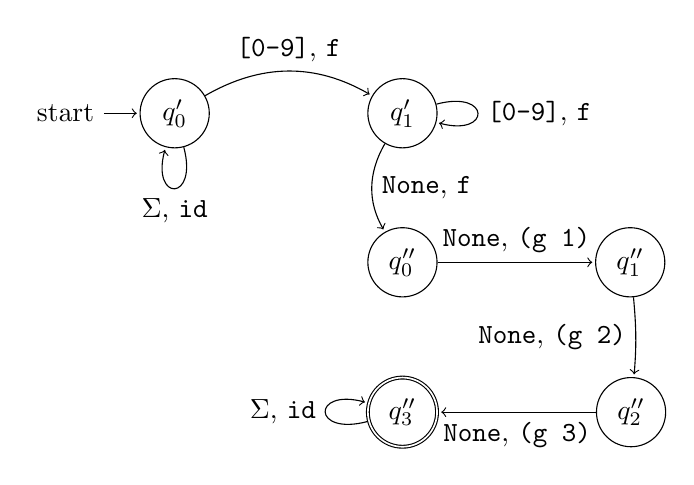
\begin{tikzpicture}[shorten >=1pt, node distance=2cm, auto]
    % Second automaton from the first figure
    \node[state, initial] (q0') {$q_0'$}; 
    \node[state] (q1') [right=of q0'] {$q_1'$}; 
  
     \path[->] 
     (q0') edge [bend left] node {\texttt{[0-9]}, $\texttt{f}$} (q1')
     (q1') edge [loop right] node {\texttt{[0-9]}, $\texttt{f}$} (q1')
     (q0') edge [loop below] node {$\Sigma$, $\texttt{id}$} (q0');
  
    % Second automaton from the second figure
    \node[state] (q0'') [below=1cm of q1'] {$q_0''$}; 
    \node[state] (q1'') [right=of q0''] {$q_1''$}; 
    \node[state, accepting] (q3'') [below=1cm of q0''] {$q_3''$}; 
    \node[state] (q2'') [right=of q3''] {$q_2''$}; 
  
    \path[->] 
    (q0'') edge node {\texttt{None}, \texttt{(g 1)}} (q1'')
    (q1'') edge [bend left=5] node[left] {\texttt{None}, \texttt{(g 2)}} (q2'')
    (q2'') edge node {\texttt{None}, \texttt{(g 3)}} (q3'')
    (q3'') edge [loop left] node {$\Sigma$, $\texttt{id}$} (q3'')
    (q1') edge [bend right=30] node {\texttt{None}, \texttt{f}} (q0'');
  \end{tikzpicture}
  \caption{The SFT for the replacement operation \\ $\texttt{replace}(s, \texttt{/[0-9]+/}, \text{``NUM''})$}
  \label{fig-rearranged-automata}
  \end{figure}


  Having constructed the SFT, we can now compute the forward image of the replacement operation. Consider the string constraint $s' = \texttt{replace}(s,~\texttt{/[0-9]+/},~\text{"}\texttt{NUM}\text{"})$, where we aim to characterize the possible values of $s'$. Let $\mathcal{T}$ denote the constructed SFT modeling the replacement operation, and let $\mathcal{A}$ be the SFA representing the domain of possible values for the input string $s$. The forward image of this replacement operation is given by the product $\mathcal{T} \times \mathcal{A}$, which precisely captures the set of all possible output strings that can be produced by applying the replacement operation to any input string accepted by $\mathcal{A}$.
  Our string solver uses this forward image to do forward propagation for further string solving.

  
  The replacement operation model described above replaces a single occurrence of any substring matching the regular expression pattern. To support different replacement semantics, 
  we model replace-all operations (which substitute all occurrences of matching substrings).

  

  The approach to modeling replace-all operations is illustrated in Figure \ref{fig:replace-all}. 



\begin{figure}[htbp]
\centering
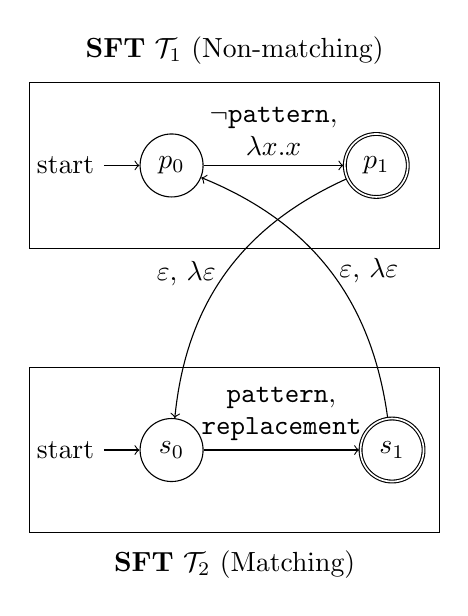
\begin{tikzpicture}[node distance=2cm, state/.style={circle, draw, minimum size=0.8cm}]
  % First SFT rectangle
  \node[draw, rectangle, minimum width=5.2cm, minimum height=2.1cm] (sft1-box) {};
  \node[above=0.1cm of sft1-box.north] {\textbf{SFT} $\mathcal{T}_1$ (Non-matching)};
  
  % States inside first SFT
  \node[state, initial] (p0) at ([xshift=-0.8cm]sft1-box.center) {$p_0$};
  \node[state, accepting] (p1) at ([xshift=1.8cm]sft1-box.center) {$p_1$};
  \path[->] (p0) edge[above] node {\shortstack{$\neg\texttt{pattern},$ \\ $\lambda x.x$}} (p1);
  
  % Second SFT rectangle
  \node[draw, rectangle, minimum width=5.2cm, minimum height=2.1cm, below=1.5cm of sft1-box] (sft2-box) {};
  \node[below=0.1cm of sft2-box.south] {\textbf{SFT} $\mathcal{T}_2$ (Matching)};
  
  % States inside second SFT
  \node[state, initial] (s0) at ([xshift=-0.8cm]sft2-box.center) {$s_0$};
  \node[state, accepting] (s1) at ([xshift=2cm]sft2-box.center) {$s_1$};
  \path[->] (s0) edge[above] node {\shortstack{$\texttt{pattern},$ \\ $\texttt{replacement}$}} (s1);
  
  % Epsilon transition from accepting state of first SFT to initial state of second SFT
  \path[->] (p1) edge[bend right=30] node[left] {\shortstack{$\varepsilon$, $\lambda\varepsilon$}} (s0);
  
  % Epsilon transition from accepting state of second SFT to initial state of first SFT
  \path[->] (s1) edge[bend right=30] node[right] {\shortstack{$\varepsilon$, $\lambda\varepsilon$}} (p0);
  
\end{tikzpicture}
\caption{The modeling of replace all operation.}
\label{fig:replace-all}
\end{figure}



\subsection{Experiments of String Replacement Operations}

We have implemented CertiStrR, an extension of  CertiStr \cite{cpp/KanLRS22}, to support string replacement operations.
%\footnote{The implementation is available at \url{https://github.com/ShlKan/certified-str-solver}}. 
CertiStr \cite{cpp/KanLRS22} is a certified string solver that only support some basic string operations, such as concatenation, and regular constraints. 


%While the core solving algorithm maintains the certification guarantees of CertiStrR, the frontend components are implemented using established non-certified  OCaml libraries: dolmen \cite{dolmen} for SMT-LIB parsing and ocaml-re-nfa \cite{ocaml-re-nfa} for regular expression to NFA conversion.

CertiStrR implements two different pattern matching introduced above: (1) singleton matching at any position, (2) replace-all matching. The pattern can be a regular expression or a constant string, which is a special case of regular expression.

% Listing \ref{lst-smtlib-code} demonstrates the regular expression variant through an example that replaces numeric sequences with the string "\texttt{NUM}". The constraints are satisfiable because the input string \texttt{a} = "\texttt{2024,2025}" contains a substring "\texttt{2025}" that matches the regular expression \texttt{re.+ (re.range "0" "9")} (equivalent to \texttt{/[0-9]+/}), and replacing this match with "\texttt{NUM}" yields the expected output string \texttt{b} = "\texttt{2024,NUM}".
% %
%
%
% \begin{lstlisting}[language=SMTLIB, caption={Example SMT-LIB Code}, label={lst-smtlib-code}, float=htbp]
%   (set-logic QF_S)
%   (declare-fun a () String)
%   (declare-fun b () String)
%   (assert (= a "2024,2025"))
%   (assert (= b "2024,NUM"))
%   (assert (= b (str.replace_re a 
%       (re.+ (re.range "0" "9")) "NUM")))
%   (check-sat)
%   \end{lstlisting}


We evaluate CertiStrR using benchmarks from SMT-LIB 2024 \cite{smtlib_benchmarks}, focusing on the QF\_S and QF\_SLIA logic fragments. The benchmarks are categorized into three groups based on their pattern matching semantics: (1) general singleton matching and (2) replace-all matching. Patterns can be either regular expressions or constant strings.

Due to CertiStrR's current frontend limitations in supporting the complete SMT-LIB language specification, we preprocess certain operations. For example, conjunctive assertions of the form \texttt{(assert (and c1 c2))} are decomposed into separate assertions \texttt{(assert c1)} and \texttt{(assert c2)} when both \texttt{c1} and \texttt{c2} are string constraints supported by CertiStrR.

% replace_re
% Average real time: 0.37 seconds
% Total number of real entries: 98
% Average user time: 0.35 seconds
% Total number of user entries: 98
% Average sys time: 0.01 seconds
% Total number of sys entries: 98
% Total number of SAT entries: 61
% Total number of UNSAT entries: 4
% Total number of inconclusive entries: 30

% replace_str
% Average real time: 0.27 seconds
% Total number of real entries: 323
% Average user time: 0.25 seconds
% Total number of user entries: 323
% Average sys time: 0.01 seconds
% Total number of sys entries: 323
% Total number of SAT entries: 315
% Total number of UNSAT entries: 173
% Total number of inconclusive entries: 8


\begin{table}[h]
  \centering
  \small
  \begin{tabular}{lcccc}
      \toprule
      & \textbf{SAT/UNSAT/Inc} & \textbf{Time (s)} & \textbf{Tests} \\
      \midrule
      \texttt{replace singleton} & 142/173/8 & 0.27 & 323\\
      \texttt{replace all} & 84/4/10 & 0.36 & 98\\
      \bottomrule
  \end{tabular}
  \caption{Experimental results}
  \label{tab:string_operations}
\end{table}

The experimental evaluation was conducted on a laptop with an Apple M4 processor and 24 GB of memory, with a one-minute time limit per test. The results show average execution times of 0.27 seconds for \texttt{replace singleton} and 0.36 seconds for \texttt{replace all}. Test outcomes were classified into three categories: SAT (satisfiable), UNSAT (unsatisfiable), and Inconclusive.

An "Inconclusive" result indicates that the solver cannot determine satisfiability, not due to timeout (all tests completed within one minute), but due to the inherent incompleteness of the string solver's algorithm. An inconclusive result can occur when the solver cannot decide whether a string variable can be assigned a unique value to make the constraints satisfiable.


Our performance analysis revealed that while the SFT-based replacement operation modeling is efficient, the primary computational bottleneck stems from automata accumulation during  forward-propagation. Consider the following string constraints:
\begin{align}
x &= x_1\texttt{++}x_2;~x = \texttt{replace}(x_3, p, r); \nonumber ~x = \texttt{replace\_re}(x_5, p_1, r_1); \nonumber
\end{align}
where \texttt{++} denotes string concatenation. The variable $x$ appears multiple times on the left-hand side of the equations, causing the forward-propagation algorithm to accumulate automata representations for all constraints: $x_1\texttt{++}x_2$, \texttt{replace}\newline($x_3, p, r$), $x_4$, and \texttt{replace\_re}($x_5, p_1, r_1$). Each accumulation step requires computing the product of the current automaton with the previous result. Given that the product operation has a worst-case complexity of $O(n^2)$, where $n$ represents the automaton size, this repeated accumulation can lead to state explosion.


\subsection{Effort of Certified Development}

This subsection discusses the development effort required for our certified SFT formalization. Table \ref{tab:abstract_impl} provides an overview of this effort.
Note that, to model replacement operation, we not only need the formalization of SFTs but also the formalization of negation of an SFA, $\epsilon$NFA.

All efforts listed in the table are additional to the existing CertiStr framework that we build upon.

The abstract-level development encompasses all formalizations presented in Sections \ref{sec:formalization} and \ref{sec:product-operation}, including SFTs and $\varepsilon$SFAs. The implementation-level development covers all formalizations in Section \ref{sec_alg_refinement}, including the refinement of the product operation. The final row corresponds to the interval formalization effort. The most challenging component proved to be the correctness proof of the product operation at the abstract level (Figure \ref{fig-def-product-correct}).

The interval formalization complexity increased dramatically in CertiStrR compared to the interval formalization in CertiStr \cite{cpp/KanLRS22}, primarily due to extending intervals from single pairs to lists.

\begin{table}[h]
  \centering
  \small
  \begin{tabular}{lccc}
      \toprule
      & \textbf{Defs} & \textbf{Lemmas} & \textbf{Proofs (LOC)} \\
      \midrule
      Abstract & 17 & 21 & 3274 \\
      Implementation & 51 & 43 & 2700 \\
      Interval & 15 & 29 & 1500 \\
      \bottomrule
  \end{tabular}
  \caption{Overview of the effort of certified development}
  \label{tab:abstract_impl}
\end{table}


\section{Related Work}
\label{sec:related-work}

\emph{Symbolic Automata and Transducers.} Symbolic Automata and Transducers \cite{cav/DAntoniV17,VeanesHLMB12Transducer, popl/DAntoniV14, entcs/DAntoniKW18, sofsem/TammV18} represent a significant advancement in automata theory, offering improved efficiency in operations and enhanced expressiveness through algebraic theories that support infinite alphabets. This symbolic framework has been progressively extended to accommodate more complex structures: symbolic tree transducers \cite{ershov/VeanesB11} handle hierarchical data structures, while symbolic pushdown automata \cite{cav/DAntoniA14} manage nested word structures. Recent developments in 2024 have further expanded the scope of symbolic techniques to include B\"{u}chi automata and omega-regular languages \cite{pacmpl/VeanesBEZ25}, enabling verification of infinite-state systems and analysis of non-terminating computations.

\emph{Applications of Symbolic Transducers.} The efficiency, scalability, and expressive power of symbolic automata and transducers have led to their widespread adoption in numerous real-world applications. These applications span diverse domains, including: constraint solving for program analysis \cite{lpar/VeanesBM10}, security-critical sanitizer analysis for web applications \cite{uss/HooimeijerLMSV11}, runtime verification of system behaviors \cite{osdi/YaseenABCL20}, and automated program inversion for software transformation \cite{pldi/HuD17}. Each application leverages the symbolic approach's ability to handle complex patterns and infinite alphabets efficiently.

\emph{Formalization of Symbolic Automata and Transducers.} While classical automata theories have been extensively formalized in interactive theorem provers \cite{Tuerk-NFA, Lammich2014TheCA, Peter14, cpp/DoczkalKS13}, with some work on transducer formalization \cite{afp/LochmannFSTS21}, the symbolic variants of automata and transducers remain largely unexplored in formal verification. To our knowledge, CertiStr \cite{cpp/KanLRS22} represents the only existing work on symbolic automata formalization in a proof assistant. Our work advances this frontier by extending the formal treatment to both SFTs and $\varepsilon$SFAs.


\emph{String Solving.} A significant application of our certified transducer framework is in string constraint solving, a field that has seen intensive research development over the past decade. While our work provides formal verification guarantees, there exists a rich ecosystem of non-certified string solvers, each with distinct capabilities: Kaluza \cite{Berkeley-JavaScript} specializes in JavaScript analysis, CVC5 \cite{cvc5}, Z3-str3 \cite{Z3-str3} builds on the Z3 framework, S3P \cite{DBLP:conf/ccs/TrinhCJ14}, Ostrich \cite{pacmpl/ChenFHHHKLRW22}, and SLOTH \cite{HJLRV18}.
As more and more bugs have beein uncovered in existing string solvers \cite{DBLP:conf/cav/BlotskyMBZKG18} and SMT solvers \cite{Mansur20} 
We believe that our work will benefit the community by providing a formal foundation for string solvers development.



\emph{Certified SMT Solvers.} Beyond string theories, certification efforts in SMT solving have extended to other domains. For example, the work by Shi et al. \cite{DBLP:conf/cav/ShiFLTWY20}, who developed a certified SMT solver for quantifier-free bit-vector theory, demonstrating the broader applicability of interactive theorem proving in certified SMT solver development.


\section{Conclusion}
\label{sec:conclusion}

We have presented the first formalization of symbolic finite transducers (SFTs)
and their most crucial algorithms in Isabelle/HOL. Our framework offers 
flexible interfaces that enable diverse applications, featuring support for 
$\varepsilon$-transitions on both inputs and outputs, as well as extensibility to various Boolean algebras through a refinement framework.
To demonstrate the practical utility of our formalization, we applied formalized
SFTs for analyzing sanitization for web applications, as well as certified 
string solving for complex constraints involving equality, concatenation,
regular constraints, and replaceall, for which we confirm the efficiency
and effectiveness of our approach on SMT-LIB 2025 benchmarks
\cite{smtlib_benchmarks}.
%We envision that our work will benefit the string solving community by 
%providing a formal foundation for string solvers development.
%from SMT-LIB 2025 \cite{smtlib_benchmarks}, and the experimental results confirm both the efficiency and effectiveness of our approach.
%applied SFTs to model string sanitization functions commonly used in web applications and showed how to verify the correctness of these sanitizers. Furthermore, we developed CertiStrR, an extension of CertiStr \cite{cpp/KanLRS22}, which adds support for string replacement operations. 




\bibliography{literature}
\end{document}